\documentclass[fleqn]{article}
\usepackage{mathtools}
\usepackage{graphicx}
\usepackage{amsmath}
\usepackage{amssymb}
\usepackage[margin = 0.25in]{geometry}
\usepackage{enumerate}
\usepackage{color}
\usepackage{fancyvrb}
\usepackage{breqn}
\usepackage{fancyhdr}
\usepackage{multicol}
%\usepackage[latin1]{inputenc}
\usepackage{tikz}\usepackage{pgfplots}
\pgfplotsset{compat=1.8}

\newcommand{\abs}[1]{\left|{#1}\right|}
\newcommand{\R}[1]{\mathbb{R}^{#1}}

\pgfplotsset{vasymptote/.style={
    before end axis/.append code={
        \draw[densely dashed] ({rel axis cs:0,0} -| {axis cs:#1,0})
        -- ({rel axis cs:0,1} -| {axis cs:#1,0});
    }
}}
\pgfplotsset{hasymptote/.style={
    before end axis/.append code={
    	%\draw (axis cs:0,1) -- ({axis cs:0,1}-|{rel axis cs:1,0});
        \draw[densely dashed] ({rel axis cs:0,1} -| {axis cs:0,#1})
        -- ({rel axis cs:0,0} -| {axis cs:0,#1});
    }
}}

\title{Exam 1 HW Solutions}

\begin{document}
{\Large\textbf{Exam 1 Homework Solutions (even problems)}}

%%%%%%%%%%%%%%%%%%%%%%%%%%%%%%%%%%%%%%%%%%%%%%%%%%%%%%%%%%%%%%%%%%%%%%%%%%
%% -------------------------- SECTION 1 ----------------------------------
%%%%%%%%%%%%%%%%%%%%%%%%%%%%%%%%%%%%%%%%%%%%%%%%%%%%%%%%%%%%%%%%%%%%%%%%%%
\section{Section 2.1}

\begin{enumerate}
\item[20)] 
\begin{align*}
f(x) &= x^2 + 2x \\
f(0) &= 0^2 + 2(0) = 0 + 0 = 0 \\
f(3) &= 3^2 + 2(3) = 9 + 6 = 15 \\
f(-3) &= (-3)^2 + 2(-3) = 9 - 6 = 3 \\
f(a) &= a^2 + 2a \\
f(-x) &= (-x)^2 + 2(-x) = x^2 - 2x \\
f\left(\frac{2}{a}\right) &= \left(\frac{1}{a}\right)^2 + 2\left(\frac{1}{a}\right) = \frac{1}{a^2} + \frac{2}{a} = \frac{1 + 2a}{a^2}
\end{align*}

\item[30)]
\begin{align*}
f(x) &= \begin{cases}
3x & \text{if } x < 0 \\
x + 1 & \text{if } 0 \leq x \leq 2 \\
(x - 2)^2 & \text{if } x > 2
\end{cases}
\end{align*}
First, find the interval for which the given $x$ value is in, and evaluate the function with the rule that applies to that $x$ value.
\begin{align*}
f(-5) &= 3(-5) = -15 \\
f(0) &= 0 + 1 = 1 \\
f(1) &= 1 + 1 = 2 \\
f(2) &= 2 + 1 = 3 \\
f(5) &= (5 - 2)^2 = 3^2 = 9
\end{align*}

\item[36)] 
\begin{align*}
f(x) &= x^2 + 1 \\
f(a) &= a^2 + 1 \\
f(a+h) &= (a + h)^2 + 1 = a^2 + 2ah + h^2 + 1 \\
\frac{f(a+h) - f(a)}{h} &= \frac{(a^2 + 2ah + h^2 + 1) - (a^2 + 1)}{h} 
= \frac{2ah + h^2}{h}
= 2a + h
\end{align*}

\item[40)]
\begin{align*}
f(x) &= \frac{2x}{x-1} \\
f(a) &= \frac{2a}{a-1} \\
f(a + h) &= \frac{2(a+h)}{a+h-1} \\ %= \frac{2a + 2h}{a + h - 1} \\
\frac{f(a+h) - f(a)}{h} &= \frac{ \frac{2(a + h)}{a + h - 1} - \frac{2a}{a-1} }{h} 
= \frac{ 2(a + h)(a-1) - 2a(a + h - 1) }{(a + h - 1)(a - 1)h}
= \frac{ 2( (a^2 + ha - a - h) - (a^2 + ha - a) )}{(a^2 + ha - a - a - h + 1)h} \\
&= \frac{ -2h }{ (a^2 + ha - 2a - h + 1)h }
= \frac{ -2 }{ a^2 + ha - 2a - h + 1 }
\end{align*}

\item[50)]
We want to worry about dividing by 0, so we need to find the $x$ values that produce a zero in the denominator:
\begin{align*}
0 &= x^2 + x - 6 = (x - 2)(x + 3) \Rightarrow x = -3, 2
\end{align*}
Any other value of $x$ will produce a real output, so the domain is
\begin{align*}
\{ x | x \not= -3, 2 \} = (-\infty, -3)\cup(-3, 2)\cup(2, \infty)
\end{align*}

\item[54)]
We know that the argument of the square root must be positive. 
We want
\begin{align*}
0 \leq 7 - 3x \Rightarrow 3x \leq 7 \Rightarrow x \leq \frac{7}{3}
\end{align*}
So the domain is $\left( -\infty, \frac{7}{3} \right]$.

\item[64)]
Again, the argument of the $4^{th}$ root must be nonnegative, and we don't want to divide by zero.
So we have
\begin{align*}
0 < 9 - x^2 \Rightarrow x^2 < 9 \Rightarrow x < 3 \text{ and } x > -3
\end{align*}
So the domain is $(-3, 3)$.

\item[72)]
\begin{enumerate}[(a)]
\item 
$D(0.1) = \sqrt{2(3960)(0.1) + (0.1)^2} = \sqrt{792.01} \approx 28.143 \quad;\quad
D(0.2) = \sqrt{2(3960)(0.2) + (0.2)^2} = \sqrt{1584.04} = 39.8$. Both measurements are in miles.

\item
Convert $h$ to miles: $h = 1135 ft (1 mi / 5280 ft) = (227/1056) mi$. So
\begin{align*}
D\left(\frac{227}{1056}\right) = \sqrt{ 2(3960)\left(\frac{227}{1056}\right) + \left( \frac{227}{1056}\right)^2 }
\approx 41.262
\end{align*}
again this is measured in miles.

\item
$D(7) = \sqrt{2(3960)(7) + 7^2} = \sqrt{55489} \approx 235.56$. So an airline pilot flying at an altitude of 7 miles can see approximately 235.56 miles of the earth ahead.

\end{enumerate}

\end{enumerate}

%%%%%%%%%%%%%%%%%%%%%%%%%%%%%%%%%%%%%%%%%%%%%%%%%%%%%%%%%%%%%%%%%%%%%%%%%%
%% -------------------------- SECTION 2 ----------------------------------
%%%%%%%%%%%%%%%%%%%%%%%%%%%%%%%%%%%%%%%%%%%%%%%%%%%%%%%%%%%%%%%%%%%%%%%%%%
\section{Section 2.2}

\begin{enumerate}
\item[8)]
\begin{tabular}{c|c}
$x$ & $f(x) = 6 - 3x$  \\ \hline
-3 & 15 \\
0 & 6 \\
2 & 0 \\
3 & -3
\end{tabular} \\
Plot: \\
\begin{tikzpicture}
\begin{axis}[
    %axis equal image,
    axis lines=middle,
    xmin=-5,xmax=5,
    ymin=-15,ymax=25,
    enlargelimits={abs=0.2cm},
    axis line style={latex-latex},
    ticklabel style={fill=white},
    ytick={-10, -5, 5, 10, 15, 20},
    xtick={-4, -3, -2, -1, 1, 2, 3, 4},
]	
	% Draw the two parts separately with individual domains:
	\addplot[samples=5,domain=-5:5, thick, color=blue, <->] {6 - 3*\x};
\end{axis}
\end{tikzpicture}

\item[12)]
\begin{tabular}{c|c}
$x$ & $f(x) = x^2 - 4$  \\ \hline
-3 & 5 \\
-2 & 0 \\
-1 & -3 \\
0 & -4 \\
1 & -3 \\
2 & 0 \\
3 & 5
\end{tabular} \\
Plot: \\
\begin{tikzpicture}
\begin{axis}[
    %axis equal image,
    axis lines=middle,
    xmin=-5,xmax=5,
    ymin=-5,ymax=10,
    enlargelimits={abs=0.2cm},
    axis line style={latex-latex},
    ticklabel style={fill=white},
    ytick={-4, -2, 2, 4, 6, 8},
    xtick={-4, -3, -2, -1, 1, 2, 3, 4},
]	
	% Draw the two parts separately with individual domains:
	\addplot[samples=50,domain=-3.5:3.5, thick, color=blue, <->] {\x^2 - 4};
\end{axis}
\end{tikzpicture}

\item[20)]
\begin{tabular}{c|c}
$x$ & $f(x) = \sqrt{x+4}$  \\ \hline
-5 & undefined \\
-4 & 0 \\
-3 & 1 \\
0 & 2 \\
5 & 3
\end{tabular} \\
Plot: \\
\begin{tikzpicture}
\begin{axis}[
    %axis equal image,
    axis lines=middle,
    xmin=-5,xmax=5,
    ymin=-1,ymax=3,
    enlargelimits={abs=0.2cm},
    axis line style={latex-latex},
    ticklabel style={fill=white},
    ytick={-0.5, 0.5, 1, 1.5, 2, 2.5},
    xtick={-4, -3, -2, -1, 1, 2, 3, 4},
]	
	% Draw the two parts separately with individual domains:
	\addplot[samples=100,domain=-4:5, thick, color=blue, ->] {(x+4)^0.5};
\end{axis}
\end{tikzpicture}

\item[36)]
\begin{align*}
f(x) &= \begin{cases}
{\color{red} 1 - x } & \text{if } x < -2 \\
{\color{blue} 5 } & \text{if } x \geq -2
\end{cases}
\end{align*}
\begin{tikzpicture}
\begin{axis}[
    %axis equal image,
    axis lines=middle,
    xmin=-5,xmax=5,
    ymin=-1,ymax=7,
    enlargelimits={abs=0.2cm},
    axis line style={latex-latex},
    ticklabel style={fill=white},
    ytick={1, 2, 3, 4, 5, 6},
    xtick={-4, -3, -2, -1, 1, 2, 3, 4},
    vasymptote=-2,
    scatter/classes={
    a={mark=o,draw=red},
    b={mark=*,blue}}
]	
	% Draw the two parts separately with individual domains:
	\addplot[samples=5,domain=-5:-2, thick, color=red, <-] {1-x};
	\addplot[samples=5,domain=-2:5, thick, color=blue, ->] {5};
	\addplot[scatter, only marks, scatter src=explicit symbolic] coordinates 		{
	(-2, 3) [a]
	(-2, 5) [b]
	};

\end{axis}
\end{tikzpicture}

\item[58)]
Solving for $y$:
\begin{align*}
3x + 7y = 21 \Rightarrow 7y = 21 - 3x \Rightarrow y = 3 - \frac{3}{7}x
\end{align*}
so the equation defines $y$ as a function of $x$.

\item[68)]
Solving for $y$:
\begin{align*}
x = y^4 \Rightarrow y = \pm\sqrt[4]{x}
\end{align*}
due to the $\pm$, this is not define $y$ as a function of $x$.

\item[70)]
\begin{enumerate}[(a)]
\item Plot:\\
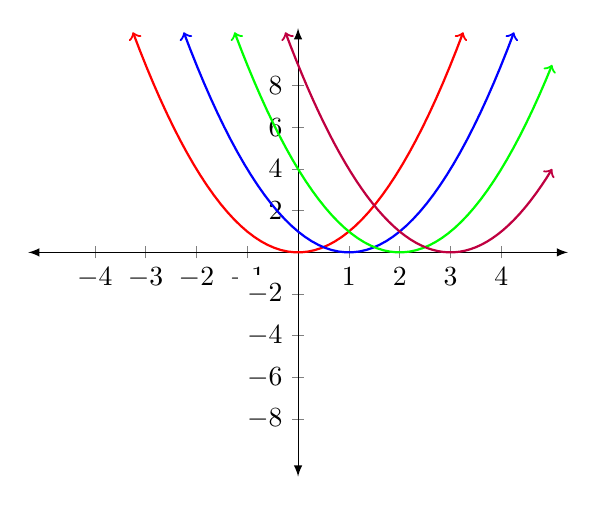
\begin{tikzpicture}
\begin{axis}[
    %axis equal image,
    axis lines=middle,
    xmin=-5,xmax=5,
    ymin=-10,ymax=10,
    enlargelimits={abs=0.2cm},
    axis line style={latex-latex},
    ticklabel style={fill=white},
    ytick={-8, -6, -4, -2, 2, 4, 6, 8},
    xtick={-4, -3, -2, -1, 1, 2, 3, 4},
    legend entries={$x^2$,$(x-1)^2$,$(x-2)^2$,$(x-3)^2$},
    legend to name=70a,
]	
	% Draw the two parts separately with individual domains:
	\addplot[samples=50,domain=-3.25:3.25, thick, color=red, <->] {x^2};
	\addplot[samples=50,domain=-2.25:4.25, thick, color=blue, <->] {(x-1)^2};
	\addplot[samples=50,domain=-1.25:5, thick, color=green, <->] {(x-2)^2};
	\addplot[samples=50,domain=-0.25:5, thick, color=purple, <->] {(x-3)^2};

\end{axis}
\end{tikzpicture}
\ref{70a}

\item Plot:\\
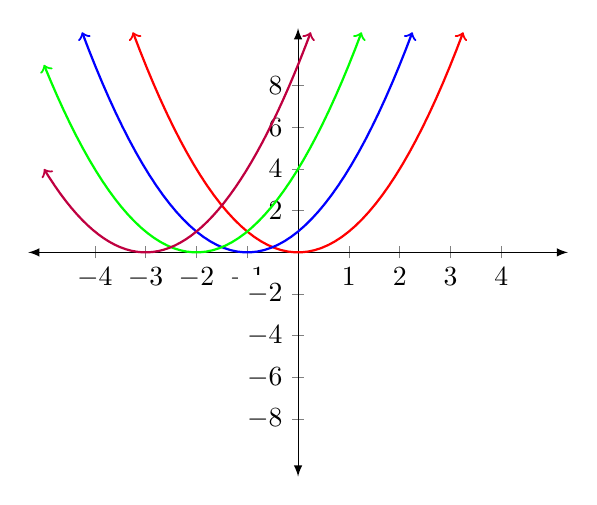
\begin{tikzpicture}
\begin{axis}[
    %axis equal image,
    axis lines=middle,
    xmin=-5,xmax=5,
    ymin=-10,ymax=10,
    enlargelimits={abs=0.2cm},
    axis line style={latex-latex},
    ticklabel style={fill=white},
    ytick={-8, -6, -4, -2, 2, 4, 6, 8},
    xtick={-4, -3, -2, -1, 1, 2, 3, 4},
    legend entries={$x^2$,$(x+1)^2$,$(x+2)^2$,$(x+3)^2$},
    legend to name=70b,
]	
	% Draw the two parts separately with individual domains:
	\addplot[samples=50,domain=-3.25:3.25, thick, color=red, <->] {x^2};
	\addplot[samples=50,domain=-4.25:2.25, thick, color=blue, <->] {(x+1)^2};
	\addplot[samples=50,domain=-5:1.25, thick, color=green, <->] {(x+2)^2};
	\addplot[samples=50,domain=-5:0.25, thick, color=purple, <->] {(x+3)^2};

\end{axis}
\end{tikzpicture}
\ref{70b}

\item $c$ shifts the graph horizontally. If $c > 0$, the graph is shifted to the right, and if $c < 0$, the graph is shifted to the left.
\end{enumerate}

\end{enumerate}

%%%%%%%%%%%%%%%%%%%%%%%%%%%%%%%%%%%%%%%%%%%%%%%%%%%%%%%%%%%%%%%%%%%%%%%%%%
%% -------------------------- SECTION 3 ----------------------------------
%%%%%%%%%%%%%%%%%%%%%%%%%%%%%%%%%%%%%%%%%%%%%%%%%%%%%%%%%%%%%%%%%%%%%%%%%%
\section{Section 2.3} 

\begin{enumerate}
\item[18)] 
\begin{enumerate}[(a)]
\item 
$f(x) = \sqrt{x+2}$. \\
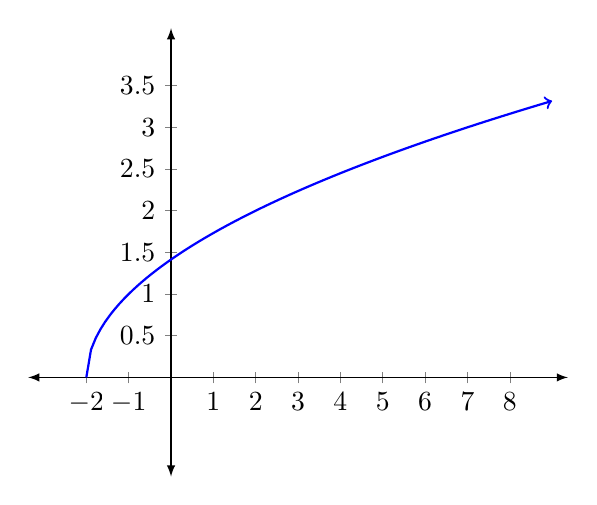
\begin{tikzpicture}
\begin{axis}[
    %axis equal image,
    axis lines=middle,
    xmin=-3,xmax=9,
    ymin=-1,ymax=4,
    enlargelimits={abs=0.2cm},
    axis line style={latex-latex},
    ticklabel style={fill=white},
    ytick={0.5, 1, 1.5, 2, 2.5, 3, 3.5},
    xtick={-2, -1, 1, 2, 3, 4, 5, 6, 7, 8},
]	
	% Draw the two parts separately with individual domains:
	\addplot[samples=100,domain=-2:9, thick, color=blue, ->] {sqrt(x+2)};
\end{axis}
\end{tikzpicture}

\item
The domain is $[-2, \infty)$.

\end{enumerate}

\item[28)]
\begin{enumerate}
\item
$f(x) = x^4 -4x^3 + 2x^2 + 4x - 3$. \\
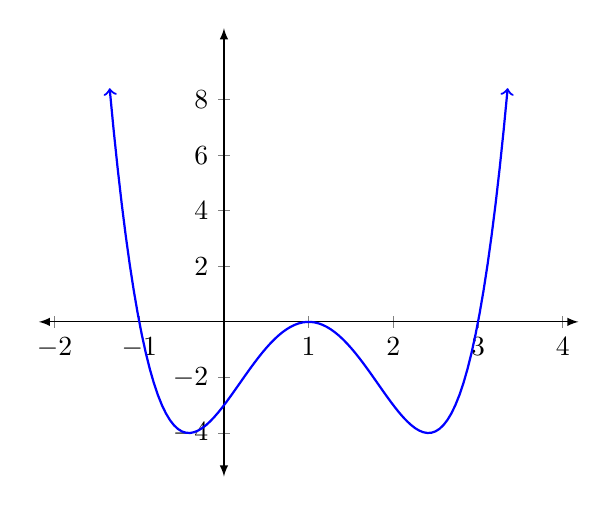
\begin{tikzpicture}
\begin{axis}[
    %axis equal image,
    axis lines=middle,
    xmin=-2,xmax=4,
    ymin=-5,ymax=10,
    enlargelimits={abs=0.2cm},
    axis line style={latex-latex},
    ticklabel style={fill=white},
    ytick={-4, -2, 2, 4, 6, 8},
    xtick={-2, -1, 1, 2, 3, 4},
]	
	% Draw the two parts separately with individual domains:
	\addplot[samples=100,domain=-1.35:3.35, thick, color=blue, <->] {x^4 -4*x^3 + 2*x^2 + 4*x - 3};
\end{axis}
\end{tikzpicture}

\item
Decreasing on $(-\infty, -0.4142]$ and $[1, 2.4142]$.
Increasing on $[-0.4142, 1]$ and $[2.4142, \infty)$.

\end{enumerate}

\item[34)]
\begin{enumerate}[(a)]
\item 
The local maxima are $3$ at $x = -2$, and $2$ at $x = 1$.
The local minima are $0$ at $x = -1$, and $-1$ at $x = 2$.

\item 
The function is increasing on the intervals $(-\infty, -2]$, $[-1, 1]$, $[2, \infty)$.
The function is decreasing on the intervals $[-2, -1]$, and $[1, 2]$.

\end{enumerate}

\item[50)]
\begin{enumerate}[(a)]
\item
$F(x) = \displaystyle \frac{350}{x^2}$ \\
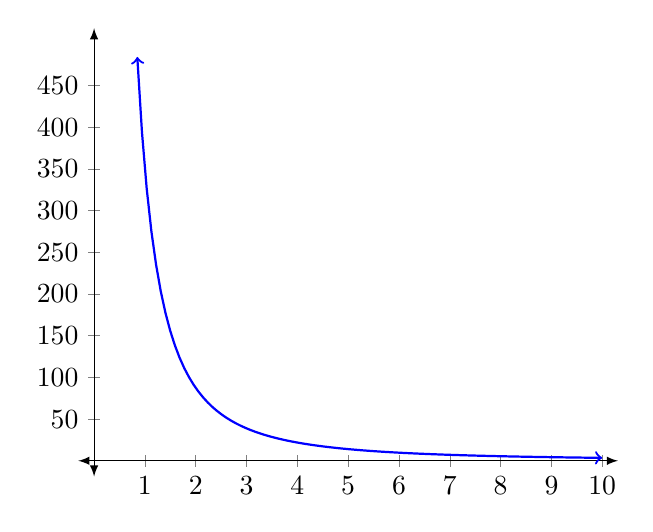
\begin{tikzpicture}
\begin{axis}[
    %axis equal image,
    axis lines=middle,
    xmin=0,xmax=10,
    ymin=0,ymax=500,
    enlargelimits={abs=0.2cm},
    axis line style={latex-latex},
    ticklabel style={fill=white},
    ytick={50, 100, 150, 200, 250, 300, 350, 400, 450},
    xtick={1, 2, 3, 4, 5, 6, 7, 8, 9, 10},
]	
	% Draw the two parts separately with individual domains:
	\addplot[samples=100,domain=0.85:10, thick, color=blue, <->] {350/x^2};
\end{axis}
\end{tikzpicture}

\item
As the distance increases, the gravitational attraction drastically decreases. In fact, the force $F$ is inversely proportional to the square of the distance $x$.

\end{enumerate}

\end{enumerate}

%%%%%%%%%%%%%%%%%%%%%%%%%%%%%%%%%%%%%%%%%%%%%%%%%%%%%%%%%%%%%%%%%%%%%%%%%%
%% -------------------------- SECTION 4 ----------------------------------
%%%%%%%%%%%%%%%%%%%%%%%%%%%%%%%%%%%%%%%%%%%%%%%%%%%%%%%%%%%%%%%%%%%%%%%%%%
\section{Section 2.4}

\begin{enumerate}
\item[8)]
The average rate of change is
\begin{align*}
\text{AROC} &= \frac{f(5) - f(-1)}{5 - (-1)}
= \frac{ 4 - 0 }{ 6 }
= \frac{2}{3}
\end{align*}

\item[18)]
The average rate of change between $x = 0$ and $x = h$ for $g(x) = \frac{2}{x+1}$ is
\begin{align*}
\text{AROC} &= \frac{g(h) - g(0)}{h - 0} 
= \frac{ \frac{2}{h+1} - \frac{2}{0+1} }{h}
= \frac{ 2 - 2(h+1)}{h(h+1)}
= \frac{ -2h }{h(h+1)}
= \frac{-2}{h+1)}
\end{align*}

\item[20)]
The average rate of change between $t = a$ and $t = a+h$ for $f(t) = \sqrt{t}$ is
\begin{align*}
\text{AROC} &= \frac{ f(a+h) - f(a) }{(a+h) - a}
= \frac{ \sqrt{a+h} - \sqrt{a} }{h} \\
&= \left( \frac{ \sqrt{a+h} - \sqrt{a} }{h} \right) \left( \frac{ \sqrt{a+h} + \sqrt{a} }{ \sqrt{a+h} + \sqrt{a} } \right)
= \frac{ \left(\sqrt{a+h}\right)^2 + \sqrt{a+h}\sqrt{a} - \sqrt{a+h}\sqrt{a} - \left(\sqrt{a}\right)^2 }{ h\left( \sqrt{a+h} + \sqrt{a} \right) } \\
&= \frac{ a+h - a }{ h\left( \sqrt{a+h} + \sqrt{a} \right) }
= \frac{ 1 }{ \left( \sqrt{a+h} + \sqrt{a} \right) }
\end{align*}
The last two lines aren't strictly necessary, but it is a simplification that you will see if you take calculus.

\end{enumerate}

%%%%%%%%%%%%%%%%%%%%%%%%%%%%%%%%%%%%%%%%%%%%%%%%%%%%%%%%%%%%%%%%%%%%%%%%%%
%% -------------------------- SECTION 5 ----------------------------------
%%%%%%%%%%%%%%%%%%%%%%%%%%%%%%%%%%%%%%%%%%%%%%%%%%%%%%%%%%%%%%%%%%%%%%%%%%
\section{Section 2.5}

\begin{enumerate}
\item[8)]
\begin{enumerate}
\item
The graph of $y = -2f(x)$ can be obtained by vertically stretching the graph of $f(x)$ by a factor of 2, and reflecting it over the $x-$axis.

\item
The graph of $y = -\frac{1}{2}f(x)$ can be obtained by vertically shrinking the graph of $f$ by a factor of 1/2, and reflecting it over the $x-$axis.

\end{enumerate}

\item[12)]
\begin{enumerate}[(a)]
\item
The graph of $y = 3 - 2f(x)$ can be obtained by first vertically stretching the graph of $f(x)$ by a factor of 2, then reflecting it over the $x-$axis, and finally shifting the graph up 3.

\item
The graph of $y = 2 - f(-x)$ can be obtained by first reflecting the graph over the $y-$axis, then over the $x-$axis, and finally shifting up by 2.

\end{enumerate}

\item[18)]
\begin{enumerate}
\item
The graph of $g(x) = -\sqrt{x} + 1$ can be obtained from $f(x) = \sqrt{x}$ by reflecting $f$ over the $x-$axis, and shifting it up 1.

\item
The graph of $g(x) = \sqrt{-x} + 1$ can be obtained from $f(x) = \sqrt{x}$ by reflecting $f$ over the $y-$axis, and shifting up 1.

\end{enumerate}

\item[34)]
The transformations are a vertical stretch by 5, and a reflection over the $x-$axis.\\
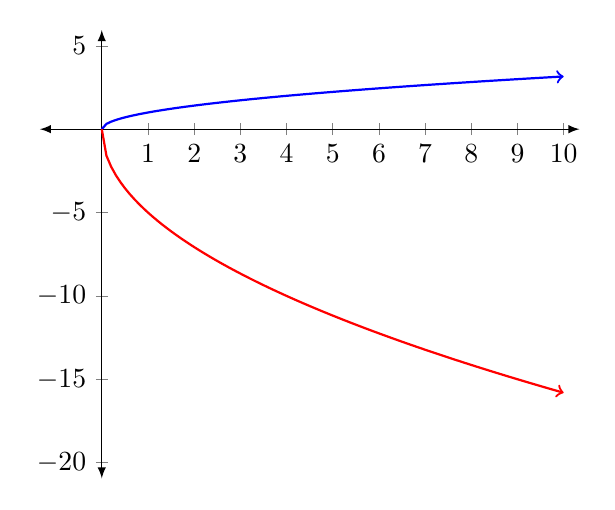
\begin{tikzpicture}
\begin{axis}[
    %axis equal image,
    axis lines=middle,
    xmin=-1,xmax=10,
    ymin=-20,ymax=5,
    enlargelimits={abs=0.2cm},
    axis line style={latex-latex},
    ticklabel style={fill=white},
    ytick={-20, -15, -10, -5, 5},
    xtick={1, 2, 3, 4, 5, 6, 7, 8, 9, 10},
    legend entries={$y = \sqrt{x}$,$y = -5\sqrt{x}$},
    legend to name=34,
]	
	% Draw the two parts separately with individual domains:
	\addplot[samples=100,domain=0:10, thick, color=blue, ->] {sqrt(x)};
	\addplot[samples=100,domain=0:10, thick, color=red, ->] {-5*sqrt(x)};
\end{axis}
\end{tikzpicture}
\ref{34}

\item[54)]
The equations step by step are
\begin{align*}
f(x) = \abs{x} \xrightarrow{\text{shrink vertically by 1/2}} \frac{1}{2} \abs{x}
\xrightarrow{\text{shift left 1}} \frac{1}{2} \abs{x+1} \xrightarrow{\text{shift up 3}} \frac{1}{2}\abs{x+1} + 3
\end{align*}

\item[66)]
Plot:\\
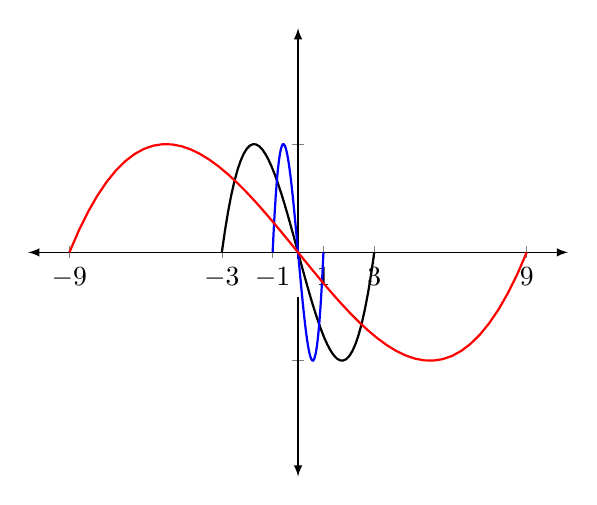
\begin{tikzpicture}
\begin{axis}[
    %axis equal image,
    axis lines=middle,
    xmin=-10,xmax=10,
    ymin=-20,ymax=20,
    enlargelimits={abs=0.2cm},
    axis line style={latex-latex},
    ticklabel style={fill=white},
    ytick={-10.4, 10.4},
    yticklabels={,},
    xtick={-9, -3, -1, 1, 3, 9},
    legend entries={$y = h(x)$, (a) $y = h(3x)$,(b) $y = h\left(\frac{1}{3}x\right)$},
    legend to name=66,
]	
	% Draw the two parts separately with individual domains:
	\addplot[samples=50,domain=-3:3, thick, color=black] {x^3 - 9*x};
	\addplot[samples=50,domain=-1:1, thick, color=blue] {27*x^3 - 27*x};
	\addplot[samples=50,domain=-9:9, thick, color=red] {x^3/27 - 3*x};
\end{axis}
\end{tikzpicture}
\ref{66}

\item[78)]
This function is definitely not odd, since tit only contains even powers of $x$, but it could be even.
We have
\begin{align*}
f(-x) &= (-x)^4 - 4(-x)^2 
= x^4 - 4x^2 
= f(x)
\end{align*}
so this is indeed an even function, and its graph is as follows.\\
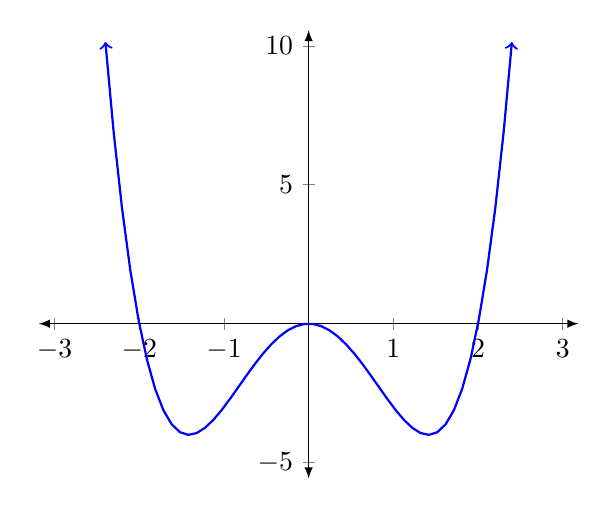
\begin{tikzpicture}
\begin{axis}[
    %axis equal image,
    axis lines=middle,
    xmin=-3,xmax=3,
    ymin=-5,ymax=10,
    enlargelimits={abs=0.2cm},
    axis line style={latex-latex},
    ticklabel style={fill=white},
    ytick={-5, 5, 10},
    xtick={-3, -2, -1, 1, 2, 3},
]	
	% Draw the two parts separately with individual domains:
	\addplot[samples=50,domain=-2.4:2.4, thick, color=blue, <->] {x^4 - 4*x^2};
\end{axis}
\end{tikzpicture}

\item[86)]
The graph of $g(x) = \abs{x^4 - 4x^2}$ looks like \\
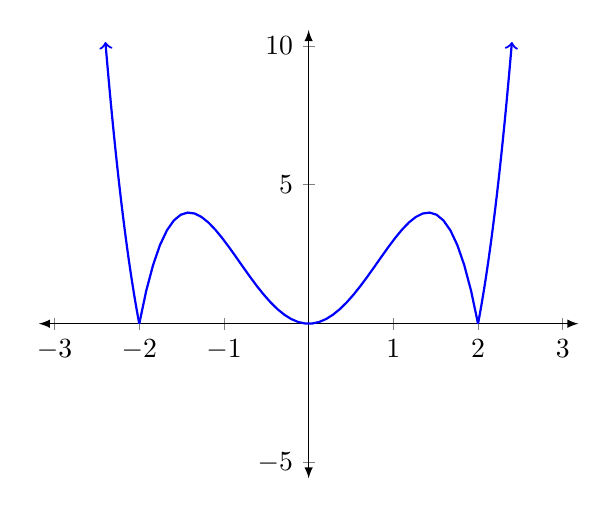
\begin{tikzpicture}
\begin{axis}[
    %axis equal image,
    axis lines=middle,
    xmin=-3,xmax=3,
    ymin=-5,ymax=10,
    enlargelimits={abs=0.2cm},
    axis line style={latex-latex},
    ticklabel style={fill=white},
    ytick={-5, 5, 10},
    xtick={-3, -2, -1, 1, 2, 3},
]	
	% Draw the two parts separately with individual domains:
	\addplot[samples=50,domain=-2.4:-2, thick, color=blue, <-] {x^4 - 4*x^2};
	\addplot[samples=50,domain=-2:2, thick, color=blue] {4*x^2 - x^4};
	\addplot[samples=50,domain=2:2.4, thick, color=blue, ->] {x^4 - 4*x^2};
\end{axis}
\end{tikzpicture}

\end{enumerate}

%%%%%%%%%%%%%%%%%%%%%%%%%%%%%%%%%%%%%%%%%%%%%%%%%%%%%%%%%%%%%%%%%%%%%%%%%%%
%%% -------------------------- SECTION 6 ----------------------------------
%%%%%%%%%%%%%%%%%%%%%%%%%%%%%%%%%%%%%%%%%%%%%%%%%%%%%%%%%%%%%%%%%%%%%%%%%%%
%\section{Section 2.6}
%
%\begin{enumerate}
%\item[10)]
%\begin{align*}
%f(x) + g(x) &= \frac{2}{x+1} + \frac{x}{x+1}
%= \frac{x + 2}{x + 1}
%\end{align*}
%
%\item[12)]
%The domain of $g(x) = \sqrt{x+1} - \frac{1}{x}$ has two constraints:
%\begin{align*}
%x + 1 \geq 0 \Rightarrow x \geq -1 \\
%x \not= 0
%\end{align*}
%Combining these, we have $[-1, 0)\cup(0,\infty)$.
%
%\item[22)]
%\begin{enumerate}[(a)]
%\item 
%$f(f(4)) = f(3(4) - 5) 
%= f(12 - 5)
%= f(7)
%= 3(7) - 5
%= 21 - 5
%= 16$
%
%\item
%$g(g(3)) = g\left( 2 - 3^2 \right)
%= g(-7)
%= 2 - (-7)^2
%= 2 - 49
%= -47$
%
%\end{enumerate}
%
%\item[30)]
%$(f\circ g)(0) = f(g(0)) = f(3) = 0$
%
%\item[32)]
%$(f\circ f)(4) = f(f(4)) = f(2) = -2$
%
%\item[44)]
%First, note that the domain of $f(x) = \frac{2}{x}$ is $(-\infty, 0)\cup(0, \infty)$.
%The domain of $g(x) = \frac{x}{x+2}$ is $(-\infty, -2)\cup(-2, \infty)$.
%The functions are
%\begin{align*}
%f\circ g &= f(g(x)) = f\left( \frac{x}{x+2} \right) = \frac{2}{ \frac{x}{x+2} }
%= \frac{ 2(x+2) }{ x } = \frac{2x + 4}{x} \\
%g\circ f &= g(f(x)) = g\left( \frac{2}{x} \right) = \frac{ 2/x }{ 2/x + 2 }
%= \frac{ 2/x }{ (2 + 2x)/x } = \left( \frac{2}{x} \right)\left( \frac{x}{2+2x} \right)
%= \frac{1}{x + 1} \\
%f\circ f &= f(f(x)) = f\left( \frac{2}{x} \right) = \frac{2}{2/x} = 2\left( \frac{x}{2} \right) = x \\
%g\circ g &= g(g(x)) = g\left( \frac{x}{x+2} \right) = \frac{x/(x+2)}{x/(x+2) + 2}
%= \frac{ x/(x+2) }{ (x + 2x + 4)/(x+2) } 
%= \left( \frac{x}{x+2} \right) \left( \frac{x+2}{3x+4} \right)
%= \frac{x}{3x+4}
%\end{align*}
%The respective domains are:
%\begin{align*}
%f\circ g: &\qquad \{ x \not= 2 \} \cap \{ g(x) \not= 0 \} 
%= \{ x \not= 2 \} \cap \left\{ \frac{x}{x+2} \not= 0 \right\} 
%= \{ x \not= 2 \} \cap \left\{ x \not= 0 \right\}
%= (-\infty, 0)\cup(0, 2)\cup(2, \infty) \\
%g\circ f: &\qquad \{ x \not= 0 \} \cap \{ f(x) \not= 0 \}
%= \{ x \not= 0 \} \cap \left\{ \frac{2}{x} \not= 0 \right\}
%= \{ x \not= 0 \} \cap \R{} 
%= (-\infty, 0)\cup(0, \infty) \\ 
%f\circ f: &\qquad \{ x \not= 0 \} \cap \{ f(x) \not= 0 \}
%= \{ x \not= 0 \} \cap \left\{ \frac{2}{x} \not= 0 \right\}
%= \{ x \not= 0 \} \cap \R{}
%= (-\infty, 0)\cup(0, \infty) \\
%g\circ g: &\qquad \{ x \not= 2 \} \cap \{ g(x) \not= 2 \}
%= \{ x \not= 2 \} \cap \left\{ \frac{x}{x+2} \not= 2 \right\}
%= \{ x \not= 2 \} \cap \{ x \not= 2x + 4 \}
%= \{ x \not= 2 \} \cap \{ -x \not= 4 \} \\
%&\hspace{1in} = \{ x \not= 2 \} \cap \{ x \not= -4 \} 
%= (-\infty, -4)\cup(-4, 2)\cup(2, \infty)
%\end{align*}
%
%\item[54)]
%Let $g(x) = \sqrt{x}$, and $f(x) = \sqrt{1 + x}$. 
%Then $H(x) = f\circ g(x) = \sqrt{1 + \sqrt{x}}$.
%
%\item[68)]
%$f\circ g(x) = f(g(x)) = f(m_2x + b_2) 
%= m_1(m2x + b_2) + b_1
%= m_1m_2x + (m_1b_2 + b_1)$.
%So $f\circ g$ is a linear function, with slope $m_1\cdot m_2$.
%
%\end{enumerate}
%
%%%%%%%%%%%%%%%%%%%%%%%%%%%%%%%%%%%%%%%%%%%%%%%%%%%%%%%%%%%%%%%%%%%%%%%%%%%
%%% -------------------------- SECTION 7 ----------------------------------
%%%%%%%%%%%%%%%%%%%%%%%%%%%%%%%%%%%%%%%%%%%%%%%%%%%%%%%%%%%%%%%%%%%%%%%%%%%
%\section{Section 2.7}
%
%\begin{enumerate}
%\item[20)]
%$f(x) = \frac{1}{x}$ is a one-to-one function, which we can see by the horizontal line test, or by noting that $f^{-1}(x) = \frac{1}{x}$ as well.
%
%\item[48)]
%\begin{align*}
%y &= \frac{ 4x - 2 }{ 3x + 1 } \Rightarrow (3x + 1)y = 4x - 2 \Rightarrow
%3xy + y = 4x - 2 \Rightarrow
%3xy - 4x = -y - 2 \Rightarrow
%(3y - 4)x = -y - 2 \Rightarrow
%x = -\frac{ y + 2 }{ 3y - 4 } \\
%&\Rightarrow f^{-1}(x) = -\frac{ x + 2 }{ 3x - 4 }
%\end{align*}
%
%\item[82)]
%\begin{enumerate}[(a)]
%\item
%\begin{align*}
%V &= 100 \left( 1 - \frac{t}{40} \right)^2 \Rightarrow
%\frac{V}{100} = \left( 1 - \frac{t}{40} \right)^2 \Rightarrow
%\frac{\sqrt{V}}{10} = 1 - \frac{t}{40} \Rightarrow
%\frac{t}{40} = 1 - \frac{\sqrt{V}}{10} \Rightarrow
%t = 40 - 4\sqrt{V}
%\end{align*}
%So $V^{-1}(t) = 40 - 4\sqrt{t}$, and it represents the time that has passed based on the volume of water in the tank.
%
%\item
%$V^{-1}(15) = 40 - 4\sqrt{15} \approx 24.5 \; min$. That is, if there is 15 gallons of water left in the tank, approximately 24.5 minutes have passed.
%
%\end{enumerate}
%
%\end{enumerate}

\end{document}